Ratio = stringent policies / permissive policies (or stringent policies when permissive policies = 0)
\begin{verbatim}
=== DMARC Policy Ratio Statistics ===
Countries with more stringent than permissive (ratio > 1): 102
Countries with more permissive than stringent (ratio <= 1): 130

Mean ratio: 1.28

Top 5 stringent countries (by ratio):
    country  ratio  stringent policies  permissive policies
81      GRL    9.0               18                 2
77      GLP    6.0               12                 2
11      ATF    5.0               10                 2
147     NER    5.0               10                 2
48      CUB    4.0               20                 5

Top 5 most permissive countries (by ratio):
    country     ratio  stringent policies  permissive policies
0       ABW  0.000000                0                 3
218     VAT  0.043478                1                23
103     JPN  0.194672             1330              6832
16      BDI  0.250000                1                 4
212     TZA  0.263736               24                91

Percent of stringent policies: 42.1%
Percent of permissive policies: 57.9%
\end{verbatim}

DMARC adoption in different continents:
\begin{verbatim}
continent	total_policies	percent_strict	percent_total
Europe	        96602	    43.838527	    64.019051
Asia	        35877	    51.909714	    52.772139
South America	18468	    54.084965	    59.945384
North America	10593	    57.226556	    60.273060
Oceania	        8203	    58.832020	    53.686613
Africa	        3731	    51.486979	    53.974564
Antarctica	    12	        83.333333	    54.545455
\end{verbatim}

The \cref{fig:stringent_policy_ratio_vs_total_policies}: strictness per nr of domains ratio. Some domains have higher absolute counts which could bias the visualization. High adoption doesn't mean high strictness (\eg Japan);
High strictness ratios usually come with low adoption;
\begin{figure}[ht]
    \centering
    \begin{subfigure}{0.48\textwidth}
        \centering
        \includegraphics[width=\linewidth]{figures/stringent_policy_ratio_vs_total_policies.pdf}
        \caption{Different countries.}
        \label{fig:stringent_policy_ratio_vs_total_policies}
    \end{subfigure}
    \hfill
    \begin{subfigure}{0.48\textwidth}
        \centering
        \includegraphics[width=\linewidth]{figures/gov_stringent_policy_ratio_vs_total_policies.pdf}
        \caption{Governmental domains.}
        \label{fig:gov_stringent_policy_ratio_vs_total_policies}
    \end{subfigure}
    \caption{Correlation between the DMARC stringent policy ratio and the total number of DMARC policies. 
    (a) Across all ccTLDs. (b) Across government domains.}
    \label{fig:ratio_vs_total_policies}
\end{figure}

\begin{figure}[ht]
    \centering
    \begin{subfigure}{0.48\textwidth}
        \centering
        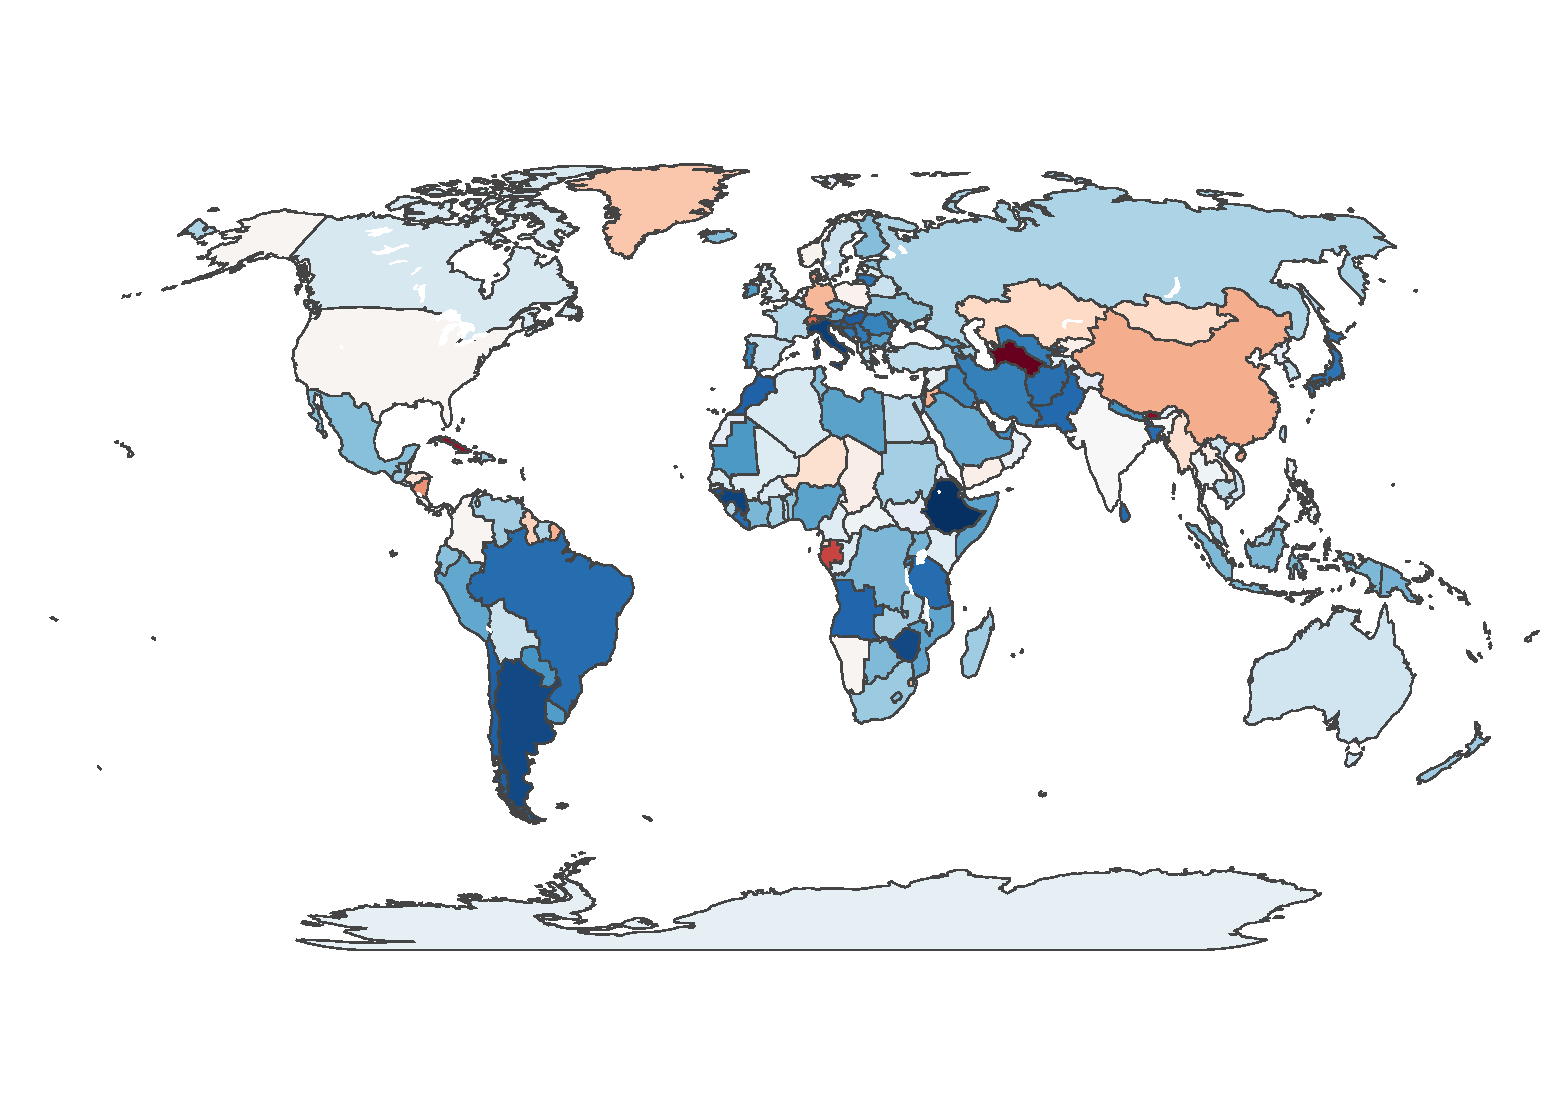
\includegraphics[width=\linewidth]{figures/world_map_stringent_policy_percentage.pdf}
        \caption{All ccTLDs.}
        \label{fig:world_map_stringent_policy_percentage}
    \end{subfigure}
    \hfill
    \begin{subfigure}{0.48\textwidth}
        \centering
        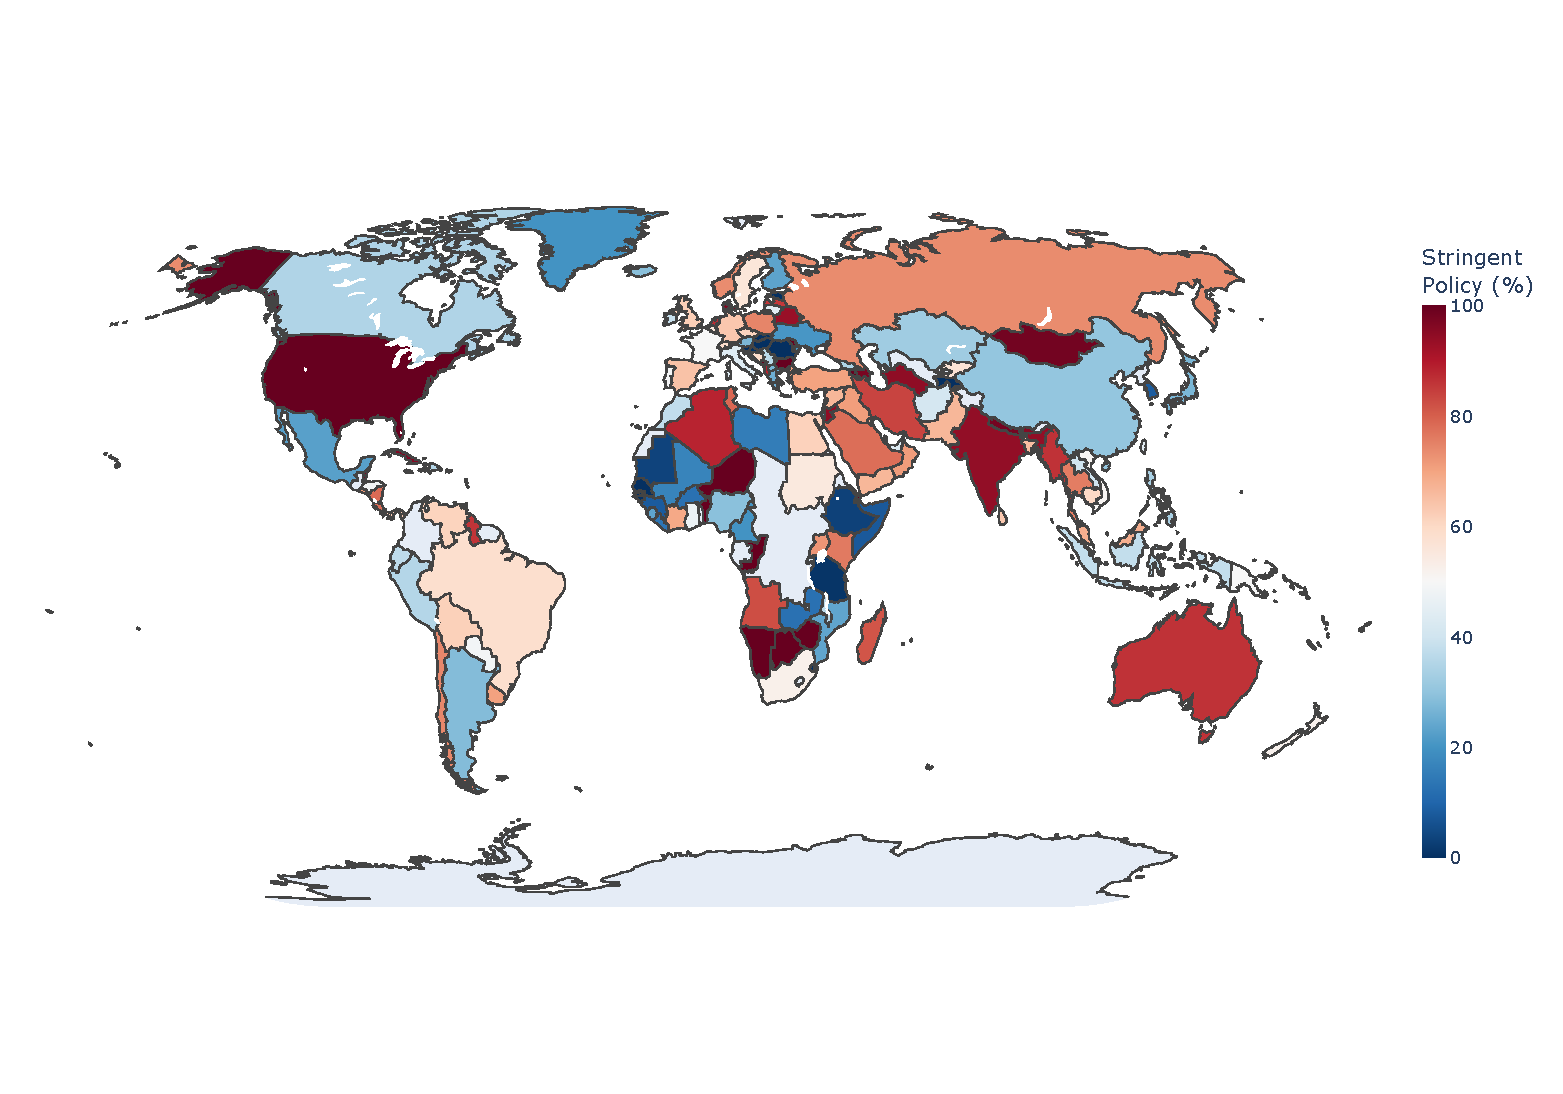
\includegraphics[width=\linewidth]{figures/gov_world_map_stringent_policy_percentage.pdf}
        \caption{Governmental domains.}
        \label{fig:gov_world_map_stringent_policy_percentage}
    \end{subfigure}
    \caption{DMARC policy distribution worldwide. 
    (a) Across all ccTLDs. (b) Across government domains.}
    \label{fig:world_map_stringent_policy_percentage_subfigures}
\end{figure}


\begin{verbatim}
=== Gov domains DMARC Policy Ratio Statistics ===
Countries with more stringent than permissive (ratio > 1): 47
Countries with more permissive than stringent (ratio <= 1): 53
Mean ratio: 2.48
Percent of stringent policies: 68.0%
Percent of permissive policies: 32.0%
\end{verbatim}

Government domains in different continents:
\begin{verbatim}
strict_policies	relaxed_policies	total_policies
continent			
Asia	1490	496	1986
North America	916	519	1435
Europe	776	261	1037
South America	394	414	808
Oceania	339	103	442
Africa	102	100	202
\end{verbatim}

Higher adoption (Five Eyes) often aligns with clearer central guidance and procurement norms; lower enforcement (EU/Intcen, BRICS) suggests operational caution—complex sender estates, third-party services, and fear of false positives.
\begin{verbatim}
=== Five Eyes Countries ===
Total DMARC policies: 23863 (73.7% adoption out of 32391 total domains within these countries)
  Stringent policies: 11058 (46.3% out of the total DMARC policies)
  Permissive policies: 12805 (53.7% out of the total DMARC policies)

=== BRICS Countries ===
Total DMARC policies: 35852 (45.6% adoption out of 78587 total domains within these countries)
  Stringent policies: 15496 (43.2% out of the total DMARC policies)
  Permissive policies: 20356 (56.8% out of the total DMARC policies)

=== EU/Intcen Countries ===
Total DMARC policies: 62573 (67.1% adoption out of 93248 total domains within these countries)
  Stringent policies: 25523 (40.8% out of the total DMARC policies)
  Permissive policies: 37050 (59.2% out of the total DMARC policies)
\end{verbatim}

\begin{table}[tb]
\footnotesize
\centering
\caption{Top 10 domains receiving DMARC reports.}
\label{tab:top_report_receivers}
\begin{tabular}{lrr}
\toprule
 & \textbf{\# reporters} & \textbf{\%} \\
\midrule
proofpoint.com & 7,297 & 6.3 \\
cloudflare.net & 6,478 & 5.6 \\
vali.email & 4,759 & 4.1 \\
dmarcanalyzer.com & 4,601 & 4.0 \\
dmarcian.com & 3,705 & 3.2 \\
brevo.com & 3,345 & 2.9 \\
dmarcadvisor.com & 3,081 & 2.7 \\
mailinblue.com & 2,791 & 2.4 \\
dmarc-report.com & 2,380 & 2.1 \\
postmarkapp.com & 2,159 & 1.9 \\
\bottomrule
\end{tabular}
\end{table}
~\cref{tab:top_report_receivers} shows the top 10 domains receiving \gls{DMARC} reports, with the amount of domains sending them report and the percentage of reporting domains that use them.
